\documentclass[border={8pt 6pt 8pt 6pt}]{standalone}
% Gemeinsamer Preamble fuer die Standalone-Grafiken der Schlusspraesentation.
% Pakete gespiegelt aus src/thesis/hslu_thesis.tex (Z. 56-60), damit die
% extrahierten TikZ-/pgfplots-Grafiken identisch zur Arbeit rendern.
\usepackage[T1]{fontenc}
\usepackage[utf8]{inputenc}
\usepackage{tikz}
\usepackage{pgfplots}
\pgfplotsset{compat=1.18}
\usepgfplotslibrary{groupplots}
\usetikzlibrary{patterns}

\begin{document}
% Extrahiert 1:1 aus chapters/05_realisierung.tex (fig:datapipeline).
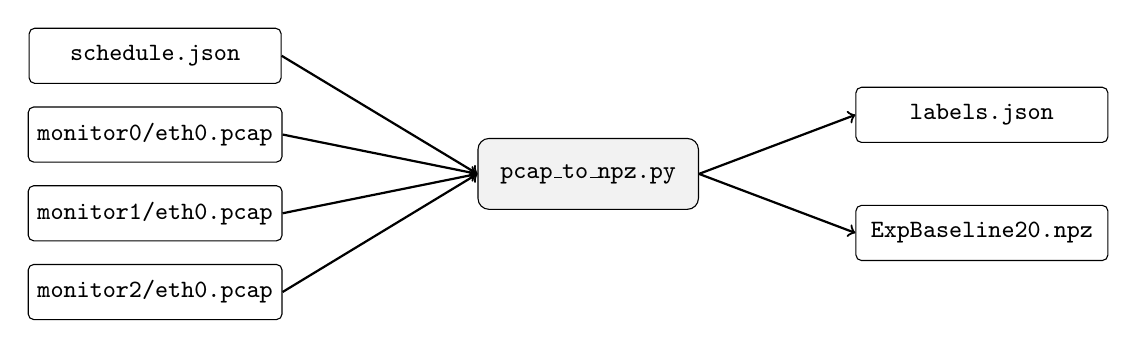
\begin{tikzpicture}[
    file/.style={draw, rounded corners=2pt, minimum width=3.2cm, minimum height=0.7cm, font=\ttfamily\small},
    script/.style={draw, rounded corners=4pt, fill=gray!10, minimum width=2.8cm, minimum height=0.9cm, font=\ttfamily\small},
    arr/.style={->, thick}
]
    \node[file]   (schedule) at (0,    0)    {schedule.json};
    \node[file]   (mon0)     at (0,   -1)    {monitor0/eth0.pcap};
    \node[file]   (mon1)     at (0,   -2)    {monitor1/eth0.pcap};
    \node[file]   (mon2)     at (0,   -3)    {monitor2/eth0.pcap};

    \node[script] (script)   at (5.5, -1.5)  {pcap\_to\_npz.py};

    \node[file]   (labels)   at (10.5,-0.75) {labels.json};
    \node[file]   (npz)      at (10.5,-2.25) {ExpBaseline20.npz};

    \draw[arr] (schedule.east) -- (script.west);
    \draw[arr] (mon0.east)     -- (script.west);
    \draw[arr] (mon1.east)     -- (script.west);
    \draw[arr] (mon2.east)     -- (script.west);

    \draw[arr] (script.east) -- (labels.west);
    \draw[arr] (script.east) -- (npz.west);
\end{tikzpicture}
\end{document}
